\documentclass[12pt]{article}

\usepackage{natbib,amsfonts,graphics,amsmath}
\usepackage{graphicx}

%
% New command file
%

% Partial Derivative
\newcommand{\D}[2]{\frac{\partial{#1}}{\partial{#2}}}
\newcommand{\dd}[2]{\frac{d{#1}}{d{#2}}}
\newcommand{\ND}[3]{\frac{\partial^{#3}{#1}}{\partial{#2}^{#3}}}
\newcommand{\DHO}[2]{\frac{\partial^H{#1}}{\partial{#2}}}
\newcommand{\de}[2]{\frac{\delta{#1}}{\delta{#2}}}
\newcommand{\deln}[3]{\frac{\delta^#3 #1}{\delta #2^#3}}
\newcommand{\SD}[2]{\frac{\partial^2{#1}}{\partial{#2}\partial{#2}}}
\newcommand{\order}[1]{\mathcal{O}\left(#1\right)}
\newcommand{\etal}{{\it\space et al. }}
\newcommand{\ub}{\mathbf{u}}
\newcommand{\fb}{\mathbf{f}}
\newcommand{\rhobar}{\overline{\rho}}
\newcommand{\xb}{\mathbf{x}}
\newcommand{\ut}{\utilde{u}}
\newcommand{\ol}[1]{\overline{#1}}
\newcommand{\twocol}[2]{\parbox{2in}{#1}\parbox{2in}{#2}}
%
% \insertfig{scalefactor}{epsfile}{caption}{label}
%
\newcommand{\insertfig}[4]{
	\begin{figure}[ht!]
	\centerline{
	\scalebox{#1}{\includegraphics{#2}}
	}
	\caption{#3}
	\label{#4}
	\end{figure}}


\begin{document}
	
	\title{The Froude number in stratified flow above topography}
	
	\author{Eric Mayer and Oliver Fringer}
	
	\maketitle
	
	\section{Abstract}
	
	There is a debate in the literature of stratified flows above topography over the correct dimensionless number to refer to as a Froude number. Common candidates include $U/ND$, $U/Nh_0$, and $Uk/N$. 
%	where $U$ is the background horizontal velocity, $N$ the background buoyancy frequency, $D$ the background depth, $h_0$ the maximum height of the topography, and $k$ a characteristic wave number of the topography. 
	Additionally, one can use the perturbation quantities $u_0$, $g'$, and $\delta$, to define an `internal' or `layer' Froude number $Fr_{\delta}=u_0/\sqrt{g'\delta}$. ~\citep{Rossby1951,Winters2012}. 
	
	In this paper, we nondimensionalize the 2D boussinesq equations describing the flow of infinitly deep fluid over topography to determine a scaling relationship between inner and outer quantities. Our scaling shows that, although it looks like an inverse Froude number, $Nh_0/U$ is in fact the square of the internal Froude number, $Fr_{\delta}^2=\frac{u_0^2}{g'\delta}$. 
	
	
	
	\section{Introduction}
	
	In its most generally accepted use, the Froude number represents a ratio of the speed with which two processes,  advection and wave propagation, carry information of a disturbance throughout a system. In the simple case of homogenous open channel flow, the Froude number is given by $Fr=q/\sqrt{gd}$, where $q$ is the  local depth-averaged velocity, $d$ is the local depth, and $g$ is the acceleration of gravity. 
	
	In the case of stratified flow with a finite depth, $D$, over a ridge of height, $h_0$, and width, $2\pi/k$, with uniform upstream velocity, $U$, and buoyancy frequency $N^2=-\frac{g}{\rho_0}\D{\bar{\rho}}{z}$ (see sketch), one can form three dimensionless numbers that resemble the Froude number, $U/ND$, $U/Nh_0$, and $Uk/N$. However, not all of these numbers represent a ratio of advection to wave propagation, and thus calling all of these parameters Froude numbers robs the concept of its intuitive dynamic significance. In his seminal text on stratified flow over topography, Baines proposed that, as a solution to this ``Froude for everything syndrome,'' the literature should only refer to the most obvious extension of open channel flow as a Froude number; that is,  $Fr=U/ND$, where $ND$ is the speed of the first mode (fastest) internal gravity wave \citep{Baines1995}. 
	
	For oceanic flows away from continents or mid-ocean ridges, however, $Fr=U/ND$ is often very small. For example, in the Drake Passage region of the Antarctic Circumpolar Current, where lee waves are predicted to be dynamically important, typical values for dimensional quantities are $U \approx 0.1$~m~s$^{-1}$, $N \approx 10^-3$~rad~s$^{-1}$, and $D \approx 4000$~m, giving $U/ND \approx 0.025$ \citep{Nikurashin2010a}. In these systems, the dynamics are captured better by considering the case of an infinitely deep ocean (e.g. \cite{Long1953}), for which solutions describe a stationary wave above the ridge, with energy propagating upwards to infinity. 
	
	In this system, the dimensionless number of primary dynamical significance is $Nh_0/U$, which has various names in the literature. Miles refers to it as the Russel number, $Ru$, after the fluid mechanician John Scott Russel, who described the reduction in drag on a shipping vessels when propelled faster than the shallow water wave speed $\sqrt{gd}$ ~\citep{Miles1969}.
%	~\footnote{ In defense of the Russel number, the dynamics of this phenomenon are more closely related to the modern conception of the Froude number than are the dynamics of the system that Froude himself considered, where the length scale was the length of the ship rather than the depth of the channel ~\citep{Baines1995}. However, rectifying history so dramatically might cause more confusion than it is worth.}
	 Aguilar and Sutherland refer to it as the Long number, $Lo$, in honor of Robert Long's pioneering work on the lee wave problem \citep{Aguilar2006a,Long1953}. Nikurashin and Ferrari refer to it as a steepness parameter and use the symbol $\epsilon$, after showing that in the hydrostatic limit, it is identical to the ratio of topographic slope to wave ray slope, an important parameter in the internal tides literature \citep{Nikurashin2010a}. And predictably, much of the literature simply refers to $Nh_0/U$ an inverse Froude number \citep{Laprise1989,Legg2008a,Klymak2010,Eckermann2010,Winters2012}. By nondimensionalizing the equations describing this flow, we will show that regardless of its name,  $Nh_0/U$ is in fact the square of the internal Froude number, $Fr_{\delta}=u_0/\sqrt{g'\delta}$. 
	
	This relation, however, breaks down if height of the topography is greater than the wavelength of the internal gravity wave, $N/U$, at which point the flow becomes hydraulically controlled, with the internal Froude number held constant at 1 \citep{Winters2012}. Thereafter, $Nh_0/U$ informs instead the degree of blocking. It is as if these hills larger than a buoyancy wavelength have squeezed all the juice out of the upstream stratified flow. Hence we term this square of an internal Froude number $J$ for Juice. 
	
	
	\section{Nondimensional equations} \label{eq:equations}
	
	\begin{figure}
		\centering
		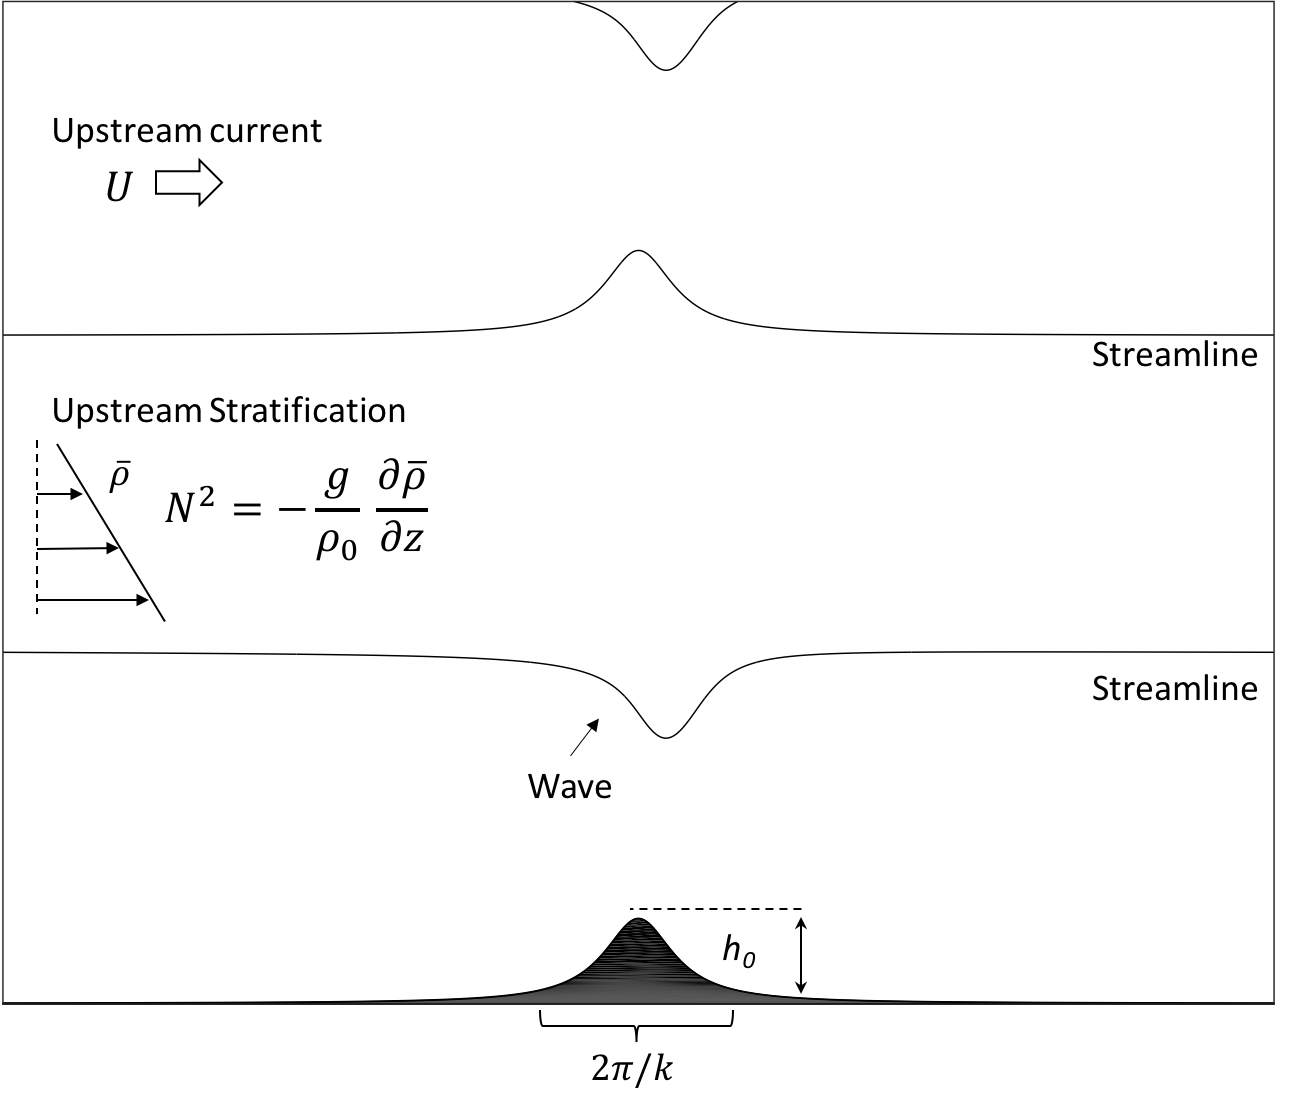
\includegraphics[width=1\textwidth]{system_sketch.png}
		\caption{Sketch of the system. Streamlines generated using the iterative solution to Long's model over a Witch of Agnesi as described in ~\cite{Laprise1989}, with $J=0.8$ and $\epsilon=0.1$. }
	\end{figure}
	
	The two-dimensional flow of an unbounded fluid over an isolated hill of height, $h_0$, and width, $2\pi/k$ is characterized by the dimensional quantities
	$U$, $k$, $N$, and $h_0$, where $U$ and $N$ are the constant horizontal velocity and buoyancy upstream of the hill. Choosing $U$ and $N$ to nondimensionalize $k$ and $h_0$, the governing
	nondimensional parameters are $J = N h_0/U$ and $\epsilon = k U/N$. 
	
	Let $\ub_{\mbox{total}} = U {\bf e}_x + \ub'$, $\rho_{\mbox{total}} = \rhobar(z) + \rho'$, and
	$p_{\mbox{total}} = \rho_0 \overline{p}(z) + \rho_0 p'$, where the prime indicates a perturbation of the field from its background state. This notation permits a rigorous separation of external (background) quantities from internal (perturbation) quantities. 
	Making the Boussinesq approximation, the steady momentum and density transport equations are given by
	\begin{eqnarray*}
	U \D{u'}{x} + \ub'\cdot\nabla u' &=& -\D{p'}{x}\,,\\
	U \D{w'}{x} + \ub'\cdot\nabla w' &=& -\D{p'}{z} - \frac{\rho'}{\rho_0} g\,,\\
	U \D{\rho'}{x} + \ub'\cdot\nabla\rho' &=& \frac{\rho_0 N^2}{g} w\,,
	\end{eqnarray*}
	where $N^2 = -g/\rho_0 \partial\rhobar/\partial z$, subject to continuity $\nabla\cdot\ub'=0$, and
	the kinematic bottom boundary condition
	\[
	U\D{h}{x} + u' \D{h}{x} = w'\,.
	\]  
	Nondimensionalize with the internal quantities
	\begin{eqnarray*}
		u' &=& u_0 u^*\,,\\
		w' &=& w_0 w^*\,,\\
		\rho' &=& R \rho^*\,,\\
		p' &=& P p^*\,,\\
		x &=& k^{-1} x^*\,,\\
		z &=& \delta z^*\,.
	\end{eqnarray*}
	Nondimensionalizing the kinematic bottom boundary condition gives
	(omitting the $*$ on nondimensional variables)
	\[
	k U h_0 \D{h}{x} + k u_0 h_0 \D{h}{x} = w_0 w\,.
	\]
	If we require a balance between the linear terms, this implies $w_0 = k h_0 U$, giving
	\[
	\D{h}{x} + \frac{u_0}{U} \D{h}{x} = w\,.
	\]
	Now, the vertical scale of the flow as given by $\delta$ is not the
	same as the hill height $h_0$, since $\delta$ must be finite as $h_0\to 0$ (the linear limit). The 
	vertical scale is thus dictated by continuity, which requires
	\[
	k u_0 \D{u}{x} + \frac{w_0}{\delta} \D{w}{z} = 0\,,
	\]
	or, since this implies $k u_0 = w_0/\delta$, then we must have $\delta = w_0/(k u_0) = k h_0 U/(k u_0) = h_0U/u_0$.
	Nondimensionalizing the $x$-momentum equation gives
	\begin{eqnarray*}
	k u_0 U \D{u}{x} + k u_0^2\ub\cdot\nabla u  &=& -k P \D{p}{x}\,.
	\end{eqnarray*}
	If we require a leading-order balance between the pressure gradient and the linear momentum advection term,
	we must have $P = u_0 U$, which gives
	\begin{eqnarray*}
	\D{u}{x} + \frac{u_0}{U} \ub\cdot\nabla u &=& -\D{p}{x}\,.
	\end{eqnarray*}
	The equation for the nondimensional density transport given by
	\[
	k U R \D{\rho}{x} + k u_0 R \ub\cdot\nabla\rho = \frac{k \rho_0 h_0 N^2 U}{g} w\,.
	\]
	If we require a balance between the linear advection terms, then the scale for the density
	perturbation is 
	\[
	R = \frac{\rho_0 N^2 h_0}{g}\,,
	\]
	so that the nondimensional density equation is
	\[
	\D{\rho}{x} + \frac{u_0}{U} \ub\cdot\nabla\rho = w\,.
	\]
	Nondimensionalizing the vertical momentum equation, we have
	\[
	k^2 h_0 U^2 \D{w}{x} + k^2 h_0 u_0^2\ub\cdot\nabla w = -\frac{P}{\delta}\D{p}{z} - \frac{g R}{\rho_0} \rho\,.
	\]
	If we require a vertical hydrostatic balance to leading order, then we must have 
	\[
	\frac{P}{\delta} = \frac{g R}{\rho_0} 
	= N^2 h_0\,,
	\]
	and
	\[
	P = \delta N^2h_0
	= \frac{N^2h_0^2U}{u_0}.
	\]
	%\[
	%P = \frac{g R \delta}{\rho_0} 
	%  = \frac{g}{\rho_0} \frac{\rho_0 N^2 h_0}{g} \frac{h_0}{F}
	%  = \frac{g}{\rho_0} \frac{\rho_0 N^2 h_0}{g} \frac{U}{N}
	%  = U N h_0\,.
	%\]
	which gives
	\[
	\epsilon^2 \left(\D{w}{x} + \frac{u_0}{U}\ub\cdot\nabla w\right) = -\D{p}{z} - \rho\,,
	\]
	where 
	\[
	\epsilon = \frac{Uk}{N}
	\]
	is the nonhydrostatic parameter, and represents a ratio of the frequency with which the flow over the hill excites a wave, $Uk$, to the frequency of the buoyant response, $N$. A propagating wave is only possible if the excitation frequency is smaller than the buoyancy frequency ($\epsilon<1$). In other words, for the perturbation from flow over a hill to result in oscillations that buoyancy can carry away from the hill, it must allow buoyancy enough time to oscillate. Within this propagating regime, one can also think of $\epsilon$ as a ratio of the wavelength of the wave to the width of the hill. For waves much smaller than the hill is long ($\epsilon<<1$), the wave is approximately hydrostatic and the group velocity of the wave (in the reference frame of the hill) is oriented vertically. 
	
	Now, returning to the pressure, since from the vertical momentum equation we
	require $P = N^2h_0^2U u_0^{-1}$ and from the horizontal momentum equation we require $P = u_0 U$, then equating the
	two implies that $u_0 = N h_0$ and thus
	\[
	\frac{u_0}{U} = \frac{N h_0}{U} \equiv J\,.
	\] 
	Therefore, in terms of $J$, the governing nondimensional equations are given by
	\begin{eqnarray*}
		\D{u}{x} + J\ub\cdot\nabla u &=& -\D{p}{x}\,,\\
		\epsilon^2 \left(\D{w}{x} + J\ub\cdot\nabla w\right) &=& -\D{p}{z} - \rho\,,\\
		\D{\rho}{x} + J \ub\cdot\nabla\rho &=& w\,,
	\end{eqnarray*}
	subject to $\nabla\cdot\ub=0$ and the kinematic bottom boundary condition
	\[
	\left(1 + J \right)\D{h}{x} = w\,.
	\]
	These nondimensional equations are consistent with the original nondimensionalization which implied
	that the problem is uniquely characterized by $\epsilon$ and $J$.
	The relevant scales (nondimensionalized by $N$ and $U$) are given by
	\begin{eqnarray*}
		\frac{u_0}{U} &=& J\,,\\
		\frac{w_0}{U} &=& \epsilon J\,,\\
		\frac{gR}{\rho_0 U N} &=& J\,,\\
		\frac{P}{U^2} &=& J\,,\\
		\frac{\delta N}{U} &=& 1\,.
	\end{eqnarray*}
	If we define the internal Froude number as
	$Fr_\delta = u_0/\sqrt{g' \delta}$, where $g'\delta =g (R/\rho_0) \delta = J U^2$, this gives
	$Fr_{\delta} = J^{1/2}$. Thus although it looks like an inverse Froude number when expressed in external variables, this scaling shows that it is
	in fact appropriate to refer to $J$ as the square of an internal Froude number. 
	
	\section{Discussion}
	
	That the outer and inner variable representations of $J$ should present velocity and gravity inversely results from the fact that the wavelength of the internal gravity wave is determined exclusively from the upstream quantities of the flow, $U$ and $N$. Dynamically, this is analogous to case of a simple pendulum, where the period of oscillation is set by the force of gravity and the length of the string, and is oblivious to the magnitude of the displacement that sets it swinging.  On the other hand, all other internal quantites in the flow scale with the ratio of the hill height to this wavelength, that is, with $J$. Thus in comparing ratios of internal advection to wave speed, the height of the hill enters linearly into the perturbation velocity, but only as a half-power in the wave speed. That is, $u_0=JU$ while $\sqrt{g'\delta} = J^{1/2} U$.  
	
	That $J$ is the square of the internal Froude number begs for an energetic interpretation of the dynamics. Borrowing from the theory of homogenous open channel flow, a flow with a set amount of energy can conceivably partition its energy into a spectrum of configurations from entirely potential ($Fr=0$) to almost entirely kinetic ($Fr \to \infty$). However, the volume flux of the flow, $Q=qd$, is not constant over this spectrum, as clearly a system with all potential energy has no flux (velocity), and a system with all kinetic energy has no volume (depth). Rather, for a given energy, the flow achieves its maximum volume flux when $Fr=1$. Similarly, our scaling shows that the perturbation volume flux, $u_0\delta$, increases with $J$ from 0 when $h_0=0$ to $U^2/N$ when $h_0=U/N$. 
	
	From the literature, however, it is clear that this the flow cannot physically sustain this maximal volume flux. A precondition on the wave solution to the flow is that it remain stable to both convective and shear instabilities ~\citep{Long1953,Miles1961}. Assymptotic and fully nonlinear solutions for the streamlines of the flow using Long's model ~\citep{Long1953} show both vertical streamlines (convective instability) and Richardson numbers smaller than 0.25 (shear instability) developing before $J$=1 for flow over a various ridge shapes (see, for example, ~\cite{Miles1969,Smith1977,Laprise1989}). Even our scaling suggests that shear instability should set in by the time $J=2$, since a reversal of flow occurs twice per wavelength, and thus $Ri\approx\frac{2g'/\delta}{(2u_0/\delta)^2}=\frac{1}{2J}$. For this reason, $J$ is generally interpreted as a nonlinearity parameter rather than the square of the internal Froude number ~\citep{Miles1969,Baines1995,Aguilar2006,Nikurashin2010a,Eckermann2010}. 
	
%	Conceptually, we can picture a column of water headed for an isolated hill. As it approaches the hill, it enters the wave field, and the lowest elements are lifted in preparation for a race across the crest. The height of this lift must be enough to overtop the hill, and scales with $h_0$. Then buoyancy acts on these lifted parcels, translating the wave's potential energy into kinetic energy. This is the source of the perturbation velocity over the hill, as indicated by the scaling $u_0=JU=Nh_0$.  This lift is also the source of the perturbation to the density field, and thus the reduced gravity that the background velocity must work against to generate the wave also scales with $h_0$. We see this in the scaling $g'=g (R/\rho_0)=JUN=N^2h_0$. However, the length scale of this work against gravity is the wavelength, $\delta$, which is oblivious to $h_0$. 
	
	Indeed, the identification of $J$ with the internal Froude number squared appears to have gone almost without notice the literature. However, an inquiry into the upper limit of this relationship recently emerged from consideration of blocked flow past a half cylinder \citep{Winters2012}. In the blocked regime, that is, for flow in which $J>O(1)$, the lowest fluid elements upstream of the obstacle lack sufficient kinetic energy to overtop the obstacle, and thus form a pool of stagnant fluid at the obstacle's base \citep{Baines1995}. As a result, the obstacle takes on the apparent height to the unblocked flow of U/N, that is, exactly the height of the flow's kinetic hill-climbing capacity, giving $J_{unblocked}=1$. In this case, Winter's and Armi show that the $Fr_{\delta}=1$ at the crest of the hill and, in analogy to hydraulic control of an unstratified river, the flow of the layer defined by the streamline that passes one wavelength above the crest of the hill exhibits a transition from subcritical flow upstream to a supercritical jet downstream followed by a dissipative hydraulic jump. 
	
	In other words, the relation between $J$ and $Fr_{\delta}$ holds only up to $J=O(1)$. Below this limit, waves accommodate the disturbance of the hill adiabatically, and carry it away from the site of generation, just as in an unstratified river flowing over a sub-critical sill. As $J$ approaches $O(1)$, the advective component of the perturbation plays a more significant role, until the perturbation volume flux above the hill reaches the maximum value that the system can energetically support. All of this squares with the dynamical significance of a Froude number. Above this limit, however, the instabilities brought on by too great a perturbation velocity restabilize the system such that the jet flowing above the hill is under hydraulic control, $Fr_{\delta}^2$=1, and $J$ informs the depth of the stagnant layer upstream as well dissipative and mixing effects of the jump downstream \citep{Winters2012}. 
	
	In this sense, the upstream characteristics of the flow present the system with a wave making capacity, and it is up top the hill to squeeze the wave into existence. But there is only so much juice in the fruit. 
	
\section{Appendix: Rotation}
Including rotation in the nondimensional equations requires only slight modification. Because rotational effects necessarily involve a spanwise direction, we must now include an equation for the spanwise momentum. 

We begin by aligning the $x$-direction with lines of latitude, and posit that the background currents are in geostrophic balance
\begin{eqnarray*}
	0 &=& -\D{P_G}{x} + fV \,,\\
	0 &=& -\D{P_G}{y} - fU \,,\\
\end{eqnarray*}
where $P_G$ is a geostrophic pressure field that is decoupled from the perturbation pressure due the lee wave. 

To keep the system as simple as possible, we further assume: it is in steady state; the bathymytery varies only in the $x$-direction; and rotation has a constant rate $f=\Omega sin(\bar{\phi})$, where $\Omega$ is the earth's rate of rotation, and $\bar{\phi}$ is the average lattitude of the domain. The assumption of steady state filters out inertial oscillations, and may be invalid in regions of the ocean where rotation is strong, such as the ACC ~\citep{Nikurashin2010a}. However, in regions closer to the equator, such as Palau, this assumption is quite good, as the following scaling analysis will demonstrate.  In combination, these three assumptions allow us to neglect all spanwise gradients in the perturbation fields because the hill only perturbs the flow in the $x$-direction, there are no inertial oscillations to deflect the flow from its hill-perturbed state, and rotation remains constant at all locations in the domain. Thus, again making the Boussinesq approximation, the steady momentum and density transport equations that include (some representation of) rotation are given by
\begin{eqnarray*}
	U \D{u'}{x} +u' \D{u'}{x} + w' \D{u'}{z} &=& -\D{p'}{x} + fv' \,,\\
	U \D{v'}{x} + u' \D{v'}{x} + w' \D{v'}{z} &=& - fu' \,,\\
	U \D{w'}{x} + u' \D{w'}{x} + w' \D{w'}{z} &=& -\D{p}{z} - \frac{\rho}{\rho_0} g \,,\\
	U \D{\rho'}{x} + u' \D{\rho'}{x} + w' \D{\rho'}{z} &=& \frac{\rho_0 N^2}{g} w\,,
\end{eqnarray*}
where $N^2 = -g/\rho_0 \partial\rhobar/\partial z$, subject to continuity $\nabla\cdot\ub'=0$, and
the kinematic bottom boundary condition
\[
U\D{h}{x} + u' \D{h}{x} = w'\,.
\]  
Note that these equations are unchanged from those in the irrotational case except for the addition of $+fv'$ to the $x$-momentum equation, and of course the presence of the $y$-momentum equation. Thus the scalings resulting from our irrotational work above hold in all cases except for these two equations. 

Nondimensionalizing as above, with the addition of $v = v_0 v*$, the $y$-momentum equation becomes
\begin{eqnarray*}
	kUv_0 \D{v}{x} + ku_0v_0\left(u \D{v}{x} + w \D{v}{z}\right) &=& - fu_0u \,.\\
\end{eqnarray*}
Requiring a balance of lowest order terms, this gives $v_0 = \frac{fu_0}{Uk}=u_0/Ro$, where $Ro = Uk/f$ is the Rossby number, and
\begin{eqnarray*}
	 \D{v}{x} + J\left(u \D{v}{x} + w \D{v}{z}\right) &=& - u \,.\\
\end{eqnarray*}
Turning next to the $x$-momentum equation, we have 
\begin{eqnarray*}
	k u_0 U \D{u}{x} + k u_0^2\left( u\D{u}{x} + w \D{u}{z}\right)  &=& -k P \D{p}{x} + fv_0v\,.
\end{eqnarray*}
Again balancing lowest order terms, we have $P=Uu_0$, and the $x$-momentum equation becomes
\begin{eqnarray*}
	\D{u}{x} +J\left( u\D{u}{x} + w \D{u}{z}\right)  &=& -\D{p}{x} + Ro^{-2}v\,.
\end{eqnarray*}	
From this result, we can diagnose the frailty of our assumptions about rotational effects. Using characteristic values of the ACC, $U \approx 0.1$~m~s$^{-1}$, $N \approx 10^-3$~rad~s$^{-1}$,  $k \approx 2\pi/2$~km, and $f\approx10^{-4}$~rad~s$^{-1}$, and $h_0\approx60$~m, we have $Ro \approx 0.5$, $Ro^{-2}\approx4$ and $J\approx 0.6$ ~\citep{Nikurashin2010a}. In other words, in the ACC, rotational effects on the scale of lee waves are zeroth order, and our assumptions simplifying them were likely misguided. However, if we focus instead on a more equatorial region with equally strong geostrophic currents, such as Palau, $f$ becomes an order of magnitude smaller, and $Ro\approx5$ for the lee wave system, giving $Ro^{-2}\approx 0.04$. Here, then, is a part of the ocean where rotation might only enter the equations as meridional jets squirting out of the lee waves.
	
	
%	reflecting hydraulic control and a local energy sink, in analogy to a hydraulic jump downstream of open channel flow over a critical height.
	
	
	
%Winters an Armi's analysis highlights an essential difference between this problem and the single layer channel flow from which our standard understanding of the Froude number derives. Consider the subcritical limit, in which $h$ is much less than $U/N$. Here the ``depth'' of the fluid as it travels over bathymetry is oblivious to both the ocean's depth and the bathymetry's height, and is instead entirely specified according to the impinging flow's properties, namely U and N. 	

%	While we would  expect a larger $N$ to block the flow and
%	reduce the magnitude of the perturbation above the hill, the scaling shows that
%	$u_0 = J U$, implying that the perturbation velocity above the sill increases in step with
%	increasing $J$. However, the gravitational force resulting from the perturbation is
%	given by $\sqrt{g'\delta} = J^{1/2} U$, which grows more slowly than $u_0$ with increasing $J$.	
	
%	(In the 2-D case, blocking is an adiabatic advective process while span wise vorticity generation and downslope winds are diabatic. In the 3-D case, horizontal splitting is an adiabatic advective response while vertical vorticity generation represents a nearly adiabatic advective non-linearity with the unique capacity to carry energy away from the site of generation.)
	



	
	%Understanding the kinetic energy in the wave is more nuanced. Beginning with the denominators in the relation $J^{1/2}=(Nh_0/U)^{1/2}=u_0/\sqrt{g'\delta}$, and multiplying $J=Nh_0/U$ by $U/U$ for dimensional consistency, we have $\sqrt{g'\delta}= U$, this expresses that the gravity wave response exists as a direct consequence of the background velocity. Indeed, in the frame of reference moving with the water, U is the magnitude of the group velocity of this wave (as both borne out in the math and evidenced by observation of the steady state hydrostatic wave standing motionless above a hill). Similarly, considering the numerators: $(Nh_0U)^{1/2}=u_0$, we see that perturbation velocity above the hill is a direct consequence of buoyancy's attempt to restore an element to its equilibrium position, where the maximum possible displacement is the height of the hill. 
	
	
	
\bibliographystyle{elsarticle-harv}
\bibliography{bibliography}
	
\end{document}